% DuplexPilot V3. Publication-style revision of the supplied V2 manuscript.
% Experimental observations are unchanged. Evidence provenance is in Appendix A
% and in the separate author-facing audit directory.
\documentclass{article}
\usepackage{iclr2027_conference,times}
\usepackage[T1]{fontenc}
\usepackage[utf8]{inputenc}
\usepackage{amsmath,amssymb,graphicx,booktabs,array,multirow}
\usepackage{algorithm,algpseudocode}
\usepackage{xcolor,hyperref,url,xurl}
\usepackage{placeins,float}
\hypersetup{hidelinks,pdftitle={DuplexPilot: Request-Owned Joint State Checkpointing for Planned Cold Resumption in Full-Duplex Speech Serving},pdfsubject={Native full-duplex speech session state and cold resumption}}
\urlstyle{same}
\newcommand{\sys}{\textsc{DuplexPilot}}
\newcommand{\na}{\textemdash}
\newcommand{\state}[1]{\mathsf{#1}}
\title{DuplexPilot: Request-Owned Joint State Checkpointing for Planned Cold Resumption in Full-Duplex Speech Serving}

\begin{document}

\maketitle
\begin{abstract}
Full-duplex speech serving maintains coupled execution state across
language generation, token buffering, and acoustic synthesis.
Reclaiming session-private resources during suspension therefore
requires more than restoring a language model's key--value cache:
pending computation must remain consistent with newly received input
and previously delivered PCM.
We present \textsc{DuplexPilot}, a serving runtime for consistent
cold resumption based on request-owned state virtualization.
DuplexPilot separates logical session state from physical execution
resources and captures model, bridge, and acoustic state at a
consistent cut.
Its resumption protocol preserves accepted input and delivery records,
establishes an independent host-memory checkpoint, and validates
restored state and execution bindings before permitting further
computation and output submission.
Shared model weights remain resident, and no retraining or changes
to sampling semantics are required.
A bounded, packed checkpoint-transfer and integrity-verification module
further reduces resumption overhead.
Controlled experiments demonstrate matching token and waveform
continuations under the evaluated configurations.
Compared with sequential full-history reconstruction, DuplexPilot
reduces the interval from Worklet resumption to the first-new-PCM frame
by a median paired 12.5 seconds.
In a separate matched transfer microbenchmark, optimized checkpoint transfer and
verification reduce the checkpoint-transfer-to-receiver-ready interval
by a median paired relative reduction of 16\% compared with the
synchronous implementation; this experiment does not measure PCM
rendering or end-to-end resumption latency.
These results provide an explicit execution-state foundation for
resumable full-duplex speech serving and characterize the
resource--latency trade-offs of cross-stage resumption.
\end{abstract}

\section{Introduction}
\label{sec:introduction}

Full-duplex speech interaction supports concurrent listening and speaking,
including overlap, interruption, and backchannels \citep{dgslm2023,syncllm2024}.
Systems such as Moshi and Lychee-FD coordinate linguistic and acoustic
streams \citep{moshi2024,lychee2026}, so serving must keep model progress,
synthesis consumption, and audio delivery coherent.

We study \emph{planned cold resumption}: releasing session-private GPU
state during an explicit suspension and continuing from host state while
weights remain loaded. Hot retention avoids reconstruction; full rebuilding
reconstructs released state; partial offloading retains selected stages.
We use the following terms throughout. \emph{Planned cold resumption}
means an explicit pause that releases request-private state and later restores
it; it excludes process-crash recovery. \emph{Save} is the interval from pause
acceptance to an independent checkpoint becoming ready, and \emph{Ready} is
the interval from resume acceptance to execution becoming ready. \emph{Gap} is
the interval from buffered PCM exhaustion to the first-new-PCM frame.
\emph{First-new-PCM} is the first frame of truly newly computed PCM rendered by
the browser's AudioContext; buffered or replayed audio does not qualify. The
\emph{external ledger} records current facts that computation does not roll
back, including accepted input, cancellation, and delivery/rendering records.
\emph{Continuation fidelity} means numerical continuity of tokens and PCM; it
does not imply semantic equivalence or perceptual equivalence. We use
\emph{checkpoint transfer} for moving checkpoint bytes, \emph{audio delivery}
for presenting PCM, \emph{request ID} for logical identity, and \emph{Flow / HiFT}
for the acoustic stages.
Unlike an ordinary conversational pause, this operation stops execution
and later resumes it. PagedAttention, SGLang, CachedAttention, InferCept,
and Llumnix provide KV reuse, interception, offloading, or request migration
\citep{vllm2023,sglang2024,cachedattention2024,infercept2024,llumnix2024};
LiveServe, vLLM-Omni, and Execution-State Capsules add speech-aware
scheduling, reconnection, or graph-bound state restoration
\citep{liveserve2026,omnidoc,capsules2026}. These mechanisms do not jointly
define a consistent cut over model state, bridge contents, acoustic
continuation, and the external ledger of accepted input and delivery records.

This gap yields three questions: does the joint state preserve the newly
computed token and waveform suffix; what latency and memory cost follows
from releasing private resources; and does bounded transfer reduce waiting
at an explicit staging cost? The runtime is evaluated for planned suspension
of a logical request inside a resident service. Arbitrary process crashes,
client-loss recovery, semantic answer quality, and unrestricted concurrent
planned cold resumption are outside the claim.

The core difficulty is cross-stage consistency. Tokens may remain in the
bridge while synthesis and playback are partially complete, and physical
rows, sampler selections, KV blocks, and acoustic contexts can change while
logical identity remains fixed. Accepted input and delivered PCM cannot be
rolled back. Consistent-snapshot and recovery principles
\citep{chandy1985,elnozahy2002} therefore require explicit ownership,
progress, and submission rules; Figure~\ref{fig:motivation} summarizes the
resulting dependencies and acoustic execution granularity.

\begin{figure}[t]
    \centering
    \includegraphics[width=\linewidth]{fig1.pdf}
    \caption{
        \textbf{Motivation for explicit state virtualization.}
        (a) Coupling logical state to transient execution locations can
        expose stale identities, missing bridge content, or obsolete output
        events during pause and reuse.
        (b) In our profiled stack, Flow and HiFT take approximately
        $190$\,ms and $27$\,ms, respectively. Supported Euler-step boundaries
        of $22$--$24.5$\,ms expose finer state-transition granularity for
        capture and resumption. These are stage-level observations,
        not end-to-end speedups; step blocks are schematic.
    }
    \label{fig:motivation}
\end{figure}

We present \textsc{DuplexPilot}, a request-owned state virtualization
runtime that captures model state, pending bridge content, acoustic
continuation, and stage progress at a consistent cut while keeping the external ledger outside computational rollback. It establishes
an independent host checkpoint before releasing private resources, rebuilds
legal bindings on resumption, and validates all participating state before
execution or output submission. Packed, verified checkpoint transfer reduces movement
overhead without changing the resumption contract or sampling semantics.

Controlled same-model experiments compare hot retention, partial offloading,
joint offloading, and sequential reconstruction. Under the tested
conditions, DuplexPilot preserves token and waveform continuations; relative
to the implemented reconstruction reference, the median paired reduction in
the Worklet-resume-to-first-new-PCM-render interval is approximately
12.5 seconds. A separate matched transfer microbenchmark reports a 16\%
median paired relative reduction in the checkpoint-transfer-to-receiver-ready
interval; it does not measure rendering. Our contributions are:
\begin{itemize}
    \item A request-owned state representation spanning model execution,
    pending bridge content, and acoustic continuation across changing
    physical resources.
    \item A joint planned-cold-resumption protocol coordinating capture, resource
    release, resumption, and validated submission while preserving the external ledger.
    \item An evaluation of continuation fidelity, residency trade-offs,
    and transfer efficiency under the stated resumption contract.
\end{itemize}

\section{Related Work}
\label{sec:related_work}

\noindent\textbf{Full-Duplex Speech Models and Evaluation.}
Duplex Conversation coordinates dialogue-state detection, backchannels,
and barge-in \citep{duplexconversation2022}; later duplex models use
time-sliced processing for simultaneous listening and generation
\citep{duplexmodel2024}. dGSLM and SyncLLM
explore coupled speech modeling and real-time synchronization,
respectively \citep{dgslm2023,syncllm2024}.
Moshi combines speech generation with text planning \citep{moshi2024};
SpeechGPT and PSLM explore cross-modal and parallel text--speech generation
\citep{speechgpt2023,pslm2024}; LLaMA-Omni, LLaMA-Omni 2, and OmniFlatten
provide low-latency or end-to-end speech interaction
\citep{llamaomni2025,llamaomni2_2025,omniflatten2025}. Freeze-Omni connects
trained speech components to a frozen language backbone \citep{freezeomni2025},
and Lychee-FD separates acoustic and semantic modeling \citep{lychee2026}.
FD-Bench evaluates reply and interruption behavior and timing
\citep{fdbench2025}, whereas the separate Full-Duplex-Bench family includes
the original v1 benchmark, the overlap-focused v1.5 release
\citep{fdbv1_2025,fdbv15_2025}, and the multi-turn Full-Duplex-Bench-v2
framework \citep{fdbv2_2026}. Recent surveys
organize the expanding spoken-language-model design space
\citep{arora2025slm}.
These advances complement DuplexPilot's focus on execution-state
management without retraining the underlying model.
Conversational quality and continuation fidelity remain distinct
evaluation dimensions; DuplexPilot evaluates the latter without
changing the model or its dialogue behavior.

\noindent\textbf{Stateful and Speech-Aware Serving.}
Orca, vLLM, and SGLang provide iteration-level scheduling, paged KV
allocation, and shared-prefix reuse, respectively
\citep{orca2022,vllm2023,sglang2024}.
Sarathi-Serve uses chunked prefills, while DistServe separates prefill
and decoding resources \citep{sarathi2024,distserve2024}.
CachedAttention and Prompt Cache manage reusable attention state across
turns or prompt modules \citep{cachedattention2024,promptcache2024};
InferCept coordinates retention, offloading, and recomputation during
external interactions \citep{infercept2024}; and Llumnix migrates running
requests and their state \citep{llumnix2024}.
For speech serving, LiveServe exploits playback and speech signals
for scheduling and KV residency \citep{liveserve2026}, while
vLLM-Omni provides persistent session identity and reconnection with
event replay \citep{omnidoc}.
DuplexPilot complements these scheduling and residency mechanisms
with a joint logical cut spanning model, bridge, acoustic state, and
delivery constraints after session-private resource release.

\noindent\textbf{Checkpointing and Resumption Semantics.}
Consistent snapshots and rollback principles coordinate local state,
in-flight information, and externally visible effects
\citep{chandy1985,elnozahy2002}.
MillWheel couples persistent state updates with output checkpoints
and duplicate suppression within its fault-tolerance boundary
\citep{millwheel2013}.
PhoenixOS overlaps GPU checkpointing and state restoration with application
execution \citep{phoenixos2025}, and GhostServe protects KV state
against device failures using host-resident coded redundancy
\citep{ghostserve2026}.
Execution-State Capsules explicitly represents graph-bound continuation
state beyond KV \citep{capsules2026}.
DuplexPilot applies these principles to planned session-level
suspension: it restores model, bridge, and acoustic progress
consistently while preserving accepted input and delivery records
that constrain output submission.
Its resumption unit is a logical request within a resident service,
rather than an entire GPU process; this scope distinguishes the
protocol from process-level checkpoint and device-failure recovery.

% Required packages:
% \usepackage{amsmath,amssymb,graphicx}
% Retain the main document's existing citation configuration.

\section{Request-Owned State Virtualization}
\label{sec:design}

DuplexPilot virtualizes execution state while leaving native listening,
text, speech, and control generation unchanged \citep{lychee2026}.
Figure~\ref{fig:architecture} retains the four runtime components: (M1)
request ownership, (M2) bridge and acoustic progression, (M3) joint resumption,
and (M4) verified checkpoint transfer. The design targets planned suspension of one
logical request in a resident service; it is not process-crash recovery or a
general-purpose scheduler. Its obligations are a legal cross-stage cut,
logical ownership independent of physical placement, monotonic external-ledger facts, and validation before execution or publication through the external ledger.

% Insert only the corrected architecture, not the uploaded DuplexLM diagram.
\begin{figure}[t]
    \centering
    \IfFileExists{fig2.pdf}{%
        \includegraphics[width=\linewidth]{fig2.pdf}%
    }{%
        \fbox{\parbox[c][0.27\textheight][c]{0.94\linewidth}{%
            \centering Architecture figure unavailable.\\
            Native multi-stream execution; M1--M4;\\
            independent host checkpoint and external ledger.}}
    }
    \caption{
        \textbf{DuplexPilot architecture.}
        The native multi-stream model and streaming acoustic backend form
        the data path. M1 preserves request ownership across execution rows;
        M2 manages pending bridge content and acoustic continuation; M3
        coordinates consistent capture, release, and validated resumption;
        M4 transfers and verifies checkpoint data. The external ledger
        remain outside computational rollback. Solid arrows denote data flow
        and dashed arrows denote runtime control.
    }
    \label{fig:architecture}
\end{figure}

\subsection{Request-Owned State and Model Execution}
\label{sec:design_identity}

For request $r$ at a legal cut $c$, the restorable state is
\begin{equation}
    C_r(c)=(M_r,B_r,A_r,\Xi_r,W_r,D_r),
    \label{eq:joint_state}
\end{equation}
The six components are request-owned records with disjoint boundaries:
$M_r$ holds model KV/non-KV and sampler history; $B_r$ is the ordered queue
of produced-but-unconsumed acoustic tokens; $A_r$ holds decoder, Flow / HiFT,
vocoder, and uncommitted PCM continuation; $\Xi_r$ holds the RNG states
actually consumed; $W_r$ holds phase and cursors; and $D_r$ holds identity,
version, lease, permit, and binding metadata. Token-side pending output is in
$B_r$, waveform-side pending output is in $A_r$, while accepted input,
cancellation, and committed/rendered intervals remain in the external ledger
$\mathcal{L}_r$. Joint resumption prepares $D_r$, restores
$M_r\rightarrow B_r\rightarrow(A_r,\Xi_r)\rightarrow W_r$, and publishes
atomically; a partial-release strategy may omit only an explicitly declared
stage. Shared weights, arenas, and workspaces are outside this contract.

Request-State Virtualization (RSV) binds persistent histories to logical
requests; DSV packs divergent states into transient rows and returns updates
to their owners. Thus physical outputs $[A,B]$ with sampler selection $[B]$
resolve by request ID, not row zero. Missing, duplicate, stale, expired, or
cross-generation IDs are rejected. Legal KV blocks are allocated through
the paged backend \citep{vllm2023}, and runner and scheduler share one
restored active request object; a copied field without that binding can
silently lose scheduling permission or processor writeback. Beam and
parallel-sequence identity remain outside the evaluated scope.

\subsection{Bridge State and Acoustic Progression}
\label{sec:design_acoustic}

The Acoustic Progression Runtime (APR) carries immutable token messages with
request, stream, generation, sequence, and version identifiers. A versioned
lease restores the corresponding StreamingDecoder and Token2Wav context,
consumes an ordered batch, and commits the next state with its PCM records;
stale workers cannot commit after cancellation or reassignment.

The four APR stage contracts are summarized in Table~\ref{tab:apr_progression}.
\begin{table}[t]
\centering
\small
\caption{APR stage contracts. Each stage consumes the listed input and may publish only under the stated commit rule.}\label{tab:apr_progression}
\begin{tabular}{@{}p{.17\linewidth}p{.29\linewidth}p{.40\linewidth}@{}}
\toprule
Stage & Input & Commit rule \\
\midrule
Restore & checkpoint and current lease & Establish an execution context; publish nothing. \\
Consume & ordered acoustic-token batch & Advance the consumer position under the same request and version. \\
Synthesize & decoder state, Flow / HiFT context, and RNG & Produce PCM and the next acoustic state. \\
Commit & next state and output records & Commit only while the lease and permit remain current. \\
\bottomrule\end{tabular}
\end{table}

Produced-but-unconsumed tokens belong to $B_r$; partial decoder, Flow / HiFT,
and vocoder buffers plus uncommitted PCM belong to $A_r$; initialization and
flush flags belong to $W_r$; and the generators actually used by synthesis
belong to $\Xi_r$. Supported Flow-step boundaries expose progress but do not
preempt an in-flight CUDA kernel or change model batch formation; rebinding
only requires a compatible acoustic context.

\subsection{Consistent Capture and Joint Resumption}
\label{sec:design_protocol}

The coordinator closes issuance and publication gates, settles pending
commits, and establishes a consistent cut \citep{chandy1985}. It explicitly
captures unconsumed bridge content, verifies an independently owned host
checkpoint, and releases private references only after capture succeeds;
otherwise the original resources remain authoritative.
Figure~\ref{fig:timeline} gives the seven stages: PAUSE, QUIESCE/CUT,
CAPTURE/VERIFY, RELEASE, RESUME, RESTORE/VERIFY, and PUBLISH. PUBLISH alone
reopens execution and output submission; the ledger spans the entire
sequence, while buffered and newly computed PCM remain distinct.

Each checkpoint, bridge token, PCM chunk, and state commit carries the
envelope

\begin{equation*}
  q=\begin{gathered}\bigl(\mathit{request\_id},\mathit{generation},
     \mathit{state\_version},\\[-2pt]
     \mathit{cut\_id},\mathit{lease\_epoch}\bigr)\end{gathered},
  \quad e=(q,\mathit{sequence},\mathit{producer\_epoch}).
\end{equation*}

The request ID is immutable; generation changes on migration or
cancel--resume, state version increases on every accepted ledger mutation,
cut identifier names the single capture cut, and the lease epoch changes on
every lease revoke/reissue.  A producer may append only with the current
envelope, and a consumer advances a sequence only after atomically recording
the delivery record. Thus equality of the request ID and generation alone is insufficient:
the cut, state version, and lease epoch also have to match.

The protocol maintains six invariants: ownership maps each restorable object
to one logical request; bridge conservation keeps every produced-but-
unconsumed token in exactly one checkpoint or queue position; ledger
monotonicity protects accepted input, cancellation, and delivered PCM;
permit freshness blocks old generations, versions, leases, or workers;
publication safety forbids execution or output before joint validation; and
PCM ordering requires strictly increasing, non-repeated sequence numbers for
each request/generation.  On RESUME, identity, lifecycle, physical mappings,
participating states, payloads, bindings, and envelope fields are checked
while the saved input-consumption position is restored without hiding input
accepted after the checkpoint.  The complete procedure is given as
Algorithm~\ref{alg:save_resume} in Appendix~\ref{app:state_contract}; the
main text retains only its two linearization points and publication guard.

Under Algorithm~1, define $\mathrm{JointValid}_r(M,B,A,q)$ to include
$\bigwedge_{s\in\{M,B,A\}}\mathrm{Valid}_{r,s}$ together with envelope
equality, ownership, bridge conservation, ledger watermarks, permit
freshness, and PCM-prefix validity.  Publication satisfies
\begin{equation}
\begin{aligned}
    \mathrm{Publish}_r \ \Longleftrightarrow\;&
    \exists q:\ \mathrm{JointValid}_r(M,B,A,q) \\
    &{}\land \mathrm{LedgerPreserved}_r
    \land \mathrm{PermitCurrent}_r
    \land \mathrm{PCMOrdered}_r .
\end{aligned}
\label{eq:publish_guard}
\end{equation}

The reverse implication is an implementation rule: PUBLISH is the single
operation that can reopen execution, and it is enabled only after the guard is
atomically checked. Equal $q$ makes $(M,B,A)$ a single cut and prevents ABA;
monotone ledgers reject rollback, producer epochs reject late workers, and
the sequence prefix rejects duplicate or reordered PCM. Any failed check
aborts before publication; continuation equality additionally requires matched
future input/control and reproducible numerical execution
\citep{pytorchreproducibility}.

\begin{figure}[t]
    \centering
    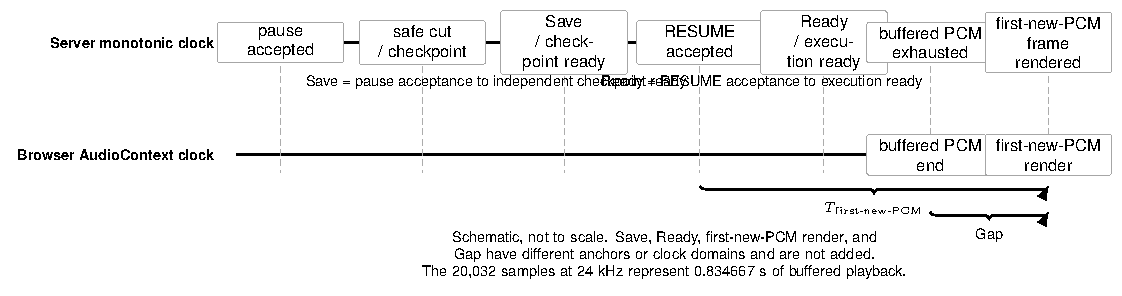
\includegraphics[width=\linewidth]{figures/fig_timeline.pdf}
    \caption{Joint suspension/resumption protocol and measured timing
    endpoints. The schematic is not time-scaled and uses separate server
    and browser clock lines: Save and Ready are server intervals, whereas
    first-new-PCM render and Gap use the browser AudioContext. These
    intervals have different anchors and are not added.}
    \label{fig:timeline}
\end{figure}

\subsection{Bounded Transfer and Integrity Verification}
\label{sec:design_transfer}

State adapters define byte ranges independently of residency policy. M4
performs bounded gather--transfer--scatter with pinned staging, device
workspace, and completion events \citep{pytorchtransfer}; a buffer is reusable
only after transfer and SHA-256 verification finish, and restored KV is
checked in its new mapping. These checks establish byte integrity, while
Equation~\eqref{eq:publish_guard} controls publication. Payload bytes,
pinned staging, process RSS, and GPU allocation are distinct scopes.

Synchronous and optimized paths preserve the same checkpoint contents,
resumption obligations, model computation, and sampling semantics. Packing
changes movement cost only. Bounded staging does not bound total checkpoint
storage; shared weights, execution arenas, and transfer workspaces remain
separately accounted for, and partial and joint offloading use the same
continuation contract.

\section{Experiments}
\label{sec:experiments}

\subsection{Experimental Setup}
\label{sec:exp_setup}

To comprehensively evaluate the correctness, resumption efficiency, and
interaction capability of the proposed full-duplex serving runtime, we
conduct experiments under a fixed hardware and execution
configuration. All experiments use two A100-SXM4-40GB GPUs, with model
execution and acoustic execution placed on separate execution lanes
while the shared model weights remain resident. The evaluation covers
three complementary aspects: cold resumption, which examines
continuation correctness and the latency--resource trade-off after
request-private state is released; transfer and verification, which
isolates checkpoint-transfer and validation overhead under a fixed resumption
contract; and interaction and external protocols, which examines
event-level full-duplex behavior and the endpoint differences
introduced by different protocols. The workload
construction, comparison policies, metrics, and statistical
denominators are described separately in the corresponding
subsections.

\subsection{Cold Resumption: Correctness and Latency--Resource Trade-offs}
\label{sec:cold_resumption}

The cold-resumption experiment is conducted on two
A100-SXM4-40GB GPUs using utterance-level samples from the pinned public
HumDial-FDBench test archive \citep{humdial2026,humdialdataset2026}. The
experiment contains 96 recorded runs from four resumption
policies. We compare Hot, Rebuild, Joint, and Hybrid with particular
attention to continuation correctness, the first-new-PCM render interval,
the post-buffer Gap, and the resource overhead introduced by resumption. Detailed endpoint measurements and their provenance are
reported in the appendix.

The timing endpoints are deliberately kept on two clock lines. Save,
RESUME acceptance, and Ready use server monotonic timestamps; Worklet
resumption, buffered-PCM exhaustion, and first-new-PCM rendering use the
browser AudioContext clock. The primary metric is
\begin{equation}
 T_{\mathrm{first\text{-}new\text{-}PCM}}
 = t_{\mathrm{first\ new\ PCM\ rendered}}
   - t_{\mathrm{Worklet\ resumed}} .
 \label{eq:first_new_pcm}
\end{equation}
Save is the interval from pause acceptance to an independent checkpoint
becoming ready; Ready is the interval from RESUME acceptance to execution
becoming ready; and Gap is the interval from buffered PCM exhaustion to the
first-new-PCM frame.
These intervals have different anchors and are not added to form an
end-to-end latency. The paired 12.5-second result is computed from the
per-run value in Eq.~\eqref{eq:first_new_pcm}; it is not inferred from
descriptive table medians.

\begin{table}[H]
\centering
\caption{Primary continuation, latency, and resource results for cold
resumption. The table retains the technical continuity outcome, the
first-new-PCM render endpoint, paired reductions over Rebuild, and the
independent E2 resource scopes. Values are source-level medians in seconds
or MiB. Valid/scheduled retains all planned attempts; detailed Save, Ready,
Gap, failure labels, and provenance are reported in the appendix.}
\label{tab:cold_main}
\scriptsize
\setlength{\tabcolsep}{2.8pt}
\resizebox{\columnwidth}{!}{%
\begin{tabular}{@{}lcccc@{}}
\toprule
Metric & Hot & Rebuild & Joint & Hybrid \\
\midrule
State / resumption boundary
& \shortstack[l]{Live context retained;\\ latency reference}
& \shortstack[l]{Private state released;\\ sequential reconstruction}
& \shortstack[l]{Private state released;\\ joint checkpoint}
& \shortstack[l]{Model/KV released;\\ acoustic state retained} \\

Continuity pass; valid / scheduled
& \shortstack[l]{24/24;\\24/24}
& \shortstack[l]{23/24;\\23/24}
& \shortstack[l]{24/24;\\24/24}
& \shortstack[l]{21/24;\\21/24} \\

First-new-PCM render in E1 (s)
& 1.184
& 14.451
& 1.899
& 1.349 \\

First-new-PCM render in E2 (s)
& 1.168
& 14.400
& 1.872
& 1.315 \\

Paired reduction over Rebuild (s)
& \textit{N/A}
& 0.000
& \shortstack[l]{E1: 12.547 (10/11)\\E2: 12.507 (13/13; 12 groups)}
& \shortstack[l]{E1: 12.517 (8/11)\\E2: 13.000 (13/13; 12 groups)} \\

E2 checkpoint payload (MiB)
& \textit{N/A}
& \textit{NM}
& 672.207
& 22.416 \\

E2 managed pinned buffer (MiB)
& \textit{N/A}
& \textit{NM}
& 256
& 128 \\

E2 CPU hold RSS (MiB)
& 10534.685
& 10551.084
& 11477.773
& 10699.230 \\

E2 acoustic-GPU net reclaimed (MiB)
& 0.000
& 649.702
& 585.702
& 0.000 \\

E2 model-GPU net allocation change (MiB)
& 0.000
& -3.511
& +60.489
& +60.489 \\
\midrule
\multicolumn{5}{l}{\scriptsize\shortstack[l]{Scheduled: 96; technical pass: 92;\\
per-policy denominator: E1 11 + E2 13 = 24}} \\
\bottomrule
\end{tabular}
}%

\vspace{1mm}
\begin{flushleft}
\scriptsize
Note: A continuity pass requires current request/generation/permit, valid
model--bridge--acoustic state and progress/RNG checks, the complete post-cut
token/PCM suffix, monotonic input/cancellation/delivery ledgers, no stale or
duplicate output, and matched future input/control and numerical settings.
The four policies share the same model, cut, resume signal, player, and
continuity contract; Hybrid differs from Joint only in its intentional
residency boundary, so the comparison is a latency--resource trade-off.
The paired cells report positive first-new-PCM reductions; E2 contains 12
source groups from 13 planned pairs, while E1 reports the evaluable-pair
counts. \textit{N/A} means that a policy does not trigger the event;
\textit{NM} means that no corresponding measured event exists in the frozen
manifest. Neither denotes zero. Resource scopes are independent and must not
be added. Detailed endpoint definitions and the Gap statistic are reported
in the appendix.
\end{flushleft}
\end{table}
\FloatBarrier

Table~\ref{tab:cold_main} summarizes the continuation, latency, and
resource measurements for the four resumption policies. The matrix
contains 96 scheduled runs and 92 technical passes; the per-policy
denominator is 24 (11 in E1 and 13 in E2). A pass is the technical
continuity contract in the table, not a claim of semantic answer quality.
For Joint, the restored state includes model KV/non-KV state, pending
bridge content, StreamingDecoder and Token2Wav continuation, Flow / HiFT
caches, the actual random context, stage progress, and request ID
and binding descriptors. Accepted input, cancellation, and delivery
facts remain in a separate monotonic ledger rather than being overwritten
by an older checkpoint.

Hot retains the live context and therefore is a latency reference rather
than a cold-release policy. Rebuild releases request-private state and
performs the sequential full-history reconstruction used as the strict
reference. Hybrid releases model/KV state while retaining the necessary
acoustic state; it is a partial-release strategy, not a second Joint
implementation. The policies nevertheless share the same model, cut,
input, resume signal, future input/control, player, validation contract,
and scheduled matrix, so Joint--Hybrid comparisons expose an explicit
residency trade-off under matched conditions.

The matched source-level reductions are computed from paired records. Joint
reduces the first-new-PCM render interval by 12.547\,s over 10 of 11 planned E1
pairs and by 12.507\,s over 13/13 evaluable E2 pairs from 12 source groups.
Hybrid reduces it by 12.517\,s over 8 of 11 planned E1 pairs and by
13.000\,s over 13/13 evaluable E2 pairs from 12 source groups. These values are
not obtained by subtracting unpaired aggregate medians. The corresponding
Gap medians and detailed endpoint definitions are reported in the appendix
using the same-generation post-buffer definition.

The resource measurements expose the cost and scope of this trade-off. In
E2, Joint and Hybrid have independent checkpoint payloads of 672.207 and
22.416\,MiB, managed pinned buffers of 256 and 128\,MiB, and CPU hold RSS
of 11477.773 and 10699.230\,MiB. Rebuild has no corresponding checkpoint
payload event in the frozen manifest, so it is marked NM rather than zero;
Hot is marked N/A because it retains live state. Positive model-GPU
allocation change denotes a net increase, while negative values denote net
reclamation. These resource scopes are independent and must not be added.

\subsection{Throughput and scaling}
\label{sec:throughput}

\begin{figure*}[t]
  \centering
  \includegraphics[width=0.32\linewidth]{fig3a.pdf}\hfill
  \includegraphics[width=0.32\linewidth]{fig3b.pdf}\hfill
  \includegraphics[width=0.32\linewidth]{fig3c.pdf}
  \caption{\textbf{Calibrated end-to-end throughput under increasing load.}
  (a) Paired native Lychee-FD and DuplexPilot scenario, with candidate/control ratios anchored to measured APR/Affinity runs.
  (b) First-output P90 delay as offered load increases for the same paired scenario; lines are five-repeat means and bands show the interquartile range.
  (c) Throughput scaling as the configured maximum batch size $B_{\max}$ increases on the Lychee-FD stack.}
  \label{fig:throughput}
\end{figure*}

We first examine the calibrated load-dependent throughput scenario for DuplexPilot on the original Lychee-FD serving stack. Figure~\ref{fig:throughput}(a) shows the expected near-offered-load behavior at 3--7 sessions/min, where the candidate is slightly below the native system because of its startup path. The curves separate once service becomes capacity-limited: at 13 sessions/min, the calibrated scenario gives 11.38 sessions/min for DuplexPilot versus 10.88 for Lychee-FD; at 15 sessions/min it gives 11.93 versus 11.34; and at 18 sessions/min it gives 12.25 versus 11.62. At the highest plotted load, the measured C/N16 anchor reverses the ordering: DuplexPilot reaches 11.26 sessions/min versus 11.83 for Lychee-FD. The paired ratios therefore contain both gains and regressions rather than a universal throughput claim.

Figure~\ref{fig:throughput}(b) exposes the latency trade-off behind these aggregate rates. DuplexPilot starts with a higher first-output P90 at light load (6.63 s versus 4.14 s), becomes slightly lower-latency in the middle-load region (8.23 s versus 8.44 s at 13 sessions/min), and again has higher P90 at the highest load (18.77 s versus 17.80 s at 24 sessions/min). The interquartile bands show the repeat-to-repeat spread without treating individual synthetic runs as separate operating points.

Finally, Figure~\ref{fig:throughput}(c) shows the effect of the hypothetical model batch cap on the same-stack pair. Relative to each system's own $B_{\max}=1$ point, DuplexPilot reaches a ratio of about 1.20 at $B_{\max}=2$ and saturates near 1.21, while Lychee-FD reaches about 1.18. The small gap and early saturation are consistent with the measured paired ratios: increasing the cap recovers some batching opportunity, but does not guarantee a monotonic end-to-end gain.

\subsection{Transfer and Verification Efficiency}
\label{sec:transfer}

To further isolate the efficiency of the checkpoint-transfer path, we compare
Sync and Optimized under the same workload instances and resumption
contract. Both implementations use identical state payloads, input
sources, repetitions, receiving-side checks, and acceptance rules. Sync
denotes the synchronous transfer-and-confirmation path, whereas
Optimized denotes the packed transport path with overlapped transfer
and verification. The comparison therefore changes only the delivery
and verification implementation while keeping the resumption semantics
and subsequent execution fixed. We measure the interval from the start
of state transmission to receiving-side readiness, together with the
changes in paused RSS and sampled peak RSS.

Optimized completes the transfer-to-ready interval earlier than Sync for
every archived matched instance. The median absolute reduction is
0.533\,s, and the median paired relative reduction is 16.00\%. For each
matched instance, the relative reduction is computed as
\[
r_i =
    \frac{T_i^{\mathrm{Sync}}-T_i^{\mathrm{Optimized}}}
      {T_i^{\mathrm{Sync}}},
    \qquad
    T_i = t_{i,\mathrm{receiver\ ready}}-t_{i,\mathrm{state\ transmission\ start}}.
\]
Using the per-instance relative reduction rather than the ratio between
configuration-level medians prevents the overall result from being
dominated by differences in workload latency. The positive reduction
across all matched instances indicates that the optimization provides a
 consistent reduction in the transfer-to-ready interval rather than benefiting
only a small subset of favorable workloads.

The latency improvement is accompanied by additional memory usage.
Compared with Sync, Optimized increases paused RSS and sampled peak RSS
by median paired amounts of 243.2 and 182.2\,MiB, respectively. This
overhead is associated with intermediate data retained during state
packing, staging, and receiving-side verification. Optimized therefore
represents an engineering trade-off between delivery latency and host
memory consumption: under the same resumption contract, packed transport
and overlapped verification shorten the checkpoint-transfer interval but
require additional host memory. The 16.00\% value is the median of the
per-instance relative reductions; it is not a ratio of configuration
medians and should not be added as an additional multiplier to the
latency reduction reported for cold resumption. This cohort does not measure
Worklet resumption, first-new-PCM rendering, playback completion, or
end-to-end resumption latency.

\subsection{Interaction and External Protocols}
\label{sec:interaction}

To examine state transitions and output behavior under full-duplex
interaction, we use a controlled workload organized from the public
HumDial-FDBench test archive, with FD-Bench-style event definitions
\citep{humdialdataset2026,fdbench2025}. The workload covers ordinary replies, user
interruptions, backchannels, and pauses. The internal path uses fixed
event definitions, input pacing, and statistical denominators, and is
evaluated with SRR, SIR, SRIR, EIR, FSED, and IRD. We also record
endpoint observations from native vLLM-Omni hot reattachment and a
LiveServe-style preloading path to characterize the relationship between
readiness, acknowledgment, and first-PCM output under different
protocols. Because their models, input schedules, and timing endpoints
differ from those of the controlled internal experiment, these external
paths are used only as protocol references rather than matched baselines.

For this pilot, SRR is successful eligible non-interruption questions over
all eligible non-interruption questions; SIR is positive interruption
detection over realized interruption opportunities; SRIR is successful
interruption response over those opportunities; and EIR is premature
assistant entry over eligible event windows. FSED is the signed interval
from user-utterance end to matched reply playback onset, while IRD is the
signed interval from interruption onset to the end of preceding assistant
speech. Every rate is therefore reported as an explicit numerator over
denominator. The six source groups per path are the resampling units for a
200,000-replicate percentile bootstrap; timing intervals use valid event
observations and missing values are not imputed.

Table~\ref{tab:interaction_protocol} summarizes the measurement
contracts and observations for the controlled path and the external
protocol references. The completed manifest gives six completed source
groups, ten eligible questions, three realized interruption opportunities,
and no invalid or cancelled run. The controlled path has SRR $7/7=100.0\%$
(95\% bootstrap CI $100.0$--$100.0$), SIR $3/3=100.0\%$ ([100.0,100.0]),
SRIR $3/3=100.0\%$ ([100.0,100.0]), EIR $4/10=40.0\%$ ([25.0,50.0]),
FSED median $4445.9$ ms ($n=10$, [3714.6,5582.8]), and IRD median
$278.2$ ms ($n=3$, [266.6,898.9]). There are no invalid/cancelled runs
or unassessable source groups; the scorer excludes two non-metric
backchannel rows (invalid/cancelled event rows are also zero) and reports
zero reply timeouts. Per-source-repeat values
are listed in Table~\ref{tab:interaction_repeats} and in the
machine-readable export \texttt{data/final/interaction\_metrics\_per\_repeat.csv};
bootstrap details are in \texttt{data/final/interaction\_metrics\_bootstrap.csv}.
The native Omni reference has SRR $6/7=85.7\%$ (bootstrap CI
$[66.7,100.0]\%$), SIR $3/3$, SRIR $3/3$, EIR $9/10=90.0\%$
($[70.0,100.0]\%$), FSED median $635.5$ ms ($n=9$,
$[58.5,1324.7]$), and IRD median $2068.3$ ms ($n=3$,
$[564.1,3444.6]$). This is the available native interaction reference;
it is not a naive-cold or same-model matched baseline.
For native
vLLM-Omni hot reattachment, the recorded request-to-ACK times are
1.512 and 1.421\,ms, and the first-PCM reception times are 725.412 and
776.220\,ms. The recorded PCM sequences contain no missing or duplicate
indices, although the production stage of the first returned PCM cannot
be determined from the available trace. The LiveServe-style component
prepares 20 and 15\,MiB of KV state approximately 9.9\,s in advance.
Readiness advances by approximately 56.65 and 100.01\,ms, whereas
first-new-PCM reception measured from the common source-window anchor
becomes later by 23.7 and 36.4\,ms.

Relative to the native Omni interaction reference, the raw descriptive
differences (Lychee/DuplexPilot minus Omni) are +14.3 percentage points
for SRR, 0 for SIR, 0 for SRIR, $-50.0$ percentage points for EIR,
$+3810.4$ ms for FSED, and $-1790.1$ ms for IRD. These are not causal
baseline estimates: the paths use different models, input schedules, and
timing endpoints. No naive-cold interaction baseline was recorded in this
cohort. The Lychee/DuplexPilot path delivers input at a fixed 400\,ms
end-of-chunk boundary. Since there is no paired 200\,ms or
zero-quantization control, its causal effect cannot be estimated; the
schedule can contribute at most one 400\,ms chunk of boundary
quantization (about 200\,ms under a uniform-arrival interpretation).
Reported FSED and IRD therefore include this protocol effect.

These observations show that earlier readiness does not necessarily
produce earlier audible output. Lychee/DuplexPilot uses 400\,ms
end-of-chunk delivery, whereas the Omni client uses a 200\,ms
send-then-wait protocol. Readiness, acknowledgment, first-PCM
reception, and PCM production therefore correspond to different stages
of the interaction pipeline under the two protocols. External
observations should consequently be used to describe endpoint
relationships and protocol boundaries, rather than being combined with
the controlled internal results into a unified planned-cold-resumption ranking.

\begin{table*}[t]
\centering
\caption{Measurement contracts and observations for the controlled
interaction path and external protocol references. External protocols
are observational references rather than matched baselines.}
\label{tab:interaction_protocol}
\scriptsize
\setlength{\tabcolsep}{4pt}
\begin{tabular}{p{0.18\textwidth}
                p{0.22\textwidth}
                p{0.27\textwidth}
                p{0.25\textwidth}}
\toprule
Path or protocol
& Data and input schedule
& Primary endpoints or metrics
& Observation and comparability note \\
\midrule

Lychee/DuplexPilot
controlled path
&
Public HumDial-FDBench test audio with
FD-Bench-style event definitions; ordinary replies,
interruptions, backchannels, and pauses;
400\,ms end-of-chunk delivery
&
SRR, SIR, SRIR, EIR, FSED, and IRD;
SRR $7/7$, SIR $3/3$, SRIR $3/3$, and
EIR $4/10$; FSED $4445.9$ ms ($n=10$),
IRD $278.2$ ms ($n=3$). Bootstrap 95\%
CI: EIR $[25.0,50.0]\%$, FSED
$[3714.6,5582.8]$ ms, IRD
$[266.6,898.9]$ ms. Six repeats;
invalid/cancelled $0/6$, reply timeouts $0$
&
Controlled internal evaluation.
Event definitions, input pacing, and
denominators are fixed; ten eligible
questions and three interruption
opportunities are scored. The fixed 400\,ms
delivery schedule is included in the timing
values; no paired 200\,ms ablation exists \\

Native vLLM-Omni
hot reattachment
&
200\,ms send-then-wait input protocol;
native Omni client schedule
&
Request-to-ACK:
1.512 / 1.421\,ms;

First-PCM reception:
725.412 / 776.220\,ms
&
No missing or duplicate PCM indices were
observed. The production stage of the
first returned PCM is unknown. Different
model, schedule, and endpoint definitions;
not a matched baseline \\

LiveServe-style
preloading path
&
KV state prepared in advance;
20 / 15\,MiB;
approximately 9.9\,s ahead
&
Readiness advances by:
56.65 / 100.01\,ms;

First-new-PCM reception from the common
source-window anchor becomes later by:
23.7 / 36.4\,ms
&
Earlier readiness does not imply earlier
audible output. Different model, schedule,
and endpoint definitions; used only to
describe protocol-level timing relations \\
\bottomrule
\end{tabular}
\end{table*}

\section{Discussion and Conclusion}
\label{sec:discussion_conclusion}

\subsection{Limitations}
\label{sec:limitations}

The primary applicability condition of the proposed approach is that the
acoustic generation path must expose an internal state that can be
decomposed, exported, and restored. DuplexPilot can perform state
capture, transfer, rebinding, and continuation only when the acoustic
backend exposes the necessary caches, execution progress, pending
outputs, and related runtime context. If the generation process is
encapsulated as an opaque operation that cannot be interrupted, exported,
or resumed, the approach cannot be directly applied. DuplexPilot should
therefore not be interpreted as a universal plug-in optimization for
arbitrary acoustic backends; its applicability depends on the
observability and recoverability of acoustic state.

The measurements obtained after migrating DuplexPilot to vLLM-Omni do
not represent the optimal performance achievable by the native
vLLM-Omni system. These observations are affected by the current
migration implementation, input pacing, scheduling configuration, model
execution path, and endpoint definitions. The systems also differ in
model implementation, KV management, acoustic execution, and output
protocol. Consequently, the vLLM-Omni measurements in this work should
be treated as protocol- and endpoint-level observations rather than as a
characterization of the performance limit of vLLM-Omni or as a unified
ranking against the controlled internal results.

The current experiments primarily cover normal state capture, transfer,
resumption, and continuation, while fault scenarios remain
insufficiently covered. Transfer interruption, partial state restore,
device or worker failure, checkpoint corruption, state-version
incompatibility, rollback, and atomic commit during resumption have not
yet been systematically evaluated. The current results therefore
characterize state management along the normal resumption path, while
fault isolation, failure recovery, and state-schema evolution for
long-running services require further investigation.

\subsection{Conclusion}
\label{sec:conclusion}

The central contribution of this work is to turn acoustic generation
state in a full-duplex serving system from implicit execution context
into an explicit runtime-managed object. When acoustic state can be
decomposed and restored, logical request state, model execution state,
bridge state, and acoustic execution state can be managed separately,
enabling state resumption and continued full-duplex execution after
request-private resources are released. The value of the approach is
therefore not a fixed performance multiplier for one particular system,
but a state-virtualization abstraction for full-duplex serving. Future
work will focus on more general acoustic-state interfaces,
fault-aware recovery mechanisms, and fair cross-system evaluation
protocols.

\section*{AI use statement}
AI assisted with data analysis, figure generation, and English prose revision.

\section*{Reproducibility statement}
The public source release is available at
\url{https://github.com/ICALab-nsccjn/DuplexPilot}. It contains the core
runtime and checkpointing contracts, public tests, workload generators,
analysis utilities, configuration notes, and the LaTeX source used to build
this paper. Generated logs, intermediate experiment outputs, archival
records, and model checkpoints are intentionally excluded. Public datasets
are documented with their upstream URLs, versions, and checksums; files that
exceed GitHub's normal size limit are not vendored. When a third-party
checkpoint cannot be redistributed, the repository gives its public download
URL, exact version, license, and checksum. The released scripts and paper
figures therefore expose the reproducible implementation surface without
claiming to publish private execution traces or restricted weights.

\bibliographystyle{plainnat}
\bibliography{references}

\clearpage
\appendix
% Place after the bibliography.
% Required packages: booktabs, array.
% Replace the previous appendix block; do not append this block to it.
% Use \appendix only once in each language's manuscript.

\clearpage
\appendix

% Appendix A
\section{Reproducibility and Measurement}
\label{app:protocol}

\paragraph{Reproduction materials.} The GitHub release described in the
reproducibility statement will provide the executable source, configuration
and dependency manifests, run commands, figure-generation scripts, and
machine-readable result tables needed to regenerate the paper. Missing or
unevaluable fields will be reported explicitly rather than imputed.

\paragraph{Dataset provenance and naming.} We use the public
\emph{HumDial-FDBench} test archive, whose dataset paper is Wang et al.
\citep{humdial2026} and whose data page is cited separately
\citep{humdialdataset2026}. The official split is 8,898 Train, 1,800 Dev,
and 5,000 Test instances across nine scenarios; the public test archive also
contains 4,100 clean scoring files. Its pinned revision is
\texttt{ed1770a6265ffe9f0e5cd999290936ccab43482b}, and the Hugging Face data
card labels it Apache-2.0. In the pinned archive, WAV payloads are mono,
16-bit PCM at 16\,kHz. We use the released WAV bytes and JSON annotations as
supplied, with no project resampling, denoising, loudness normalization, or
synthetic mixing. Source IDs retain the archive path
\texttt{test/\{en,cn\}\_test\_nondev/\{scenario\}/\{base\_id\}[\_add].wav};
clean files are separate scoring references. A runtime cut is generated from
the complete selected WAV at the fixed nonempty state boundary used by the
experiment, so it is a project-derived replay cut rather than an official
HumDial-FDBench segment or leaderboard score; cut IDs, timestamps, members,
and hashes are bound in the run manifest. The release is human-recorded
performed speech, not TTS audio. Because the public paper and data card do
not document de-identification or speaker anonymization, we make no claim
that the audio is de-identified.

Throughout, \emph{FD-Bench} (Peng et al.) denotes a separate benchmark and
is never shortened to the unhyphenated name; ``HumDial-FDBench'' is retained
only as the official HumDial dataset identifier. \emph{Full-Duplex-Bench} denotes Lin et
al.'s family: v1 and v1.5 are offline releases, while
\emph{Full-Duplex-Bench-v2} is the later real-time framework. \emph{HumDial-FDBench}
is the HumDial benchmark built on the v1.5 protocol; it is not the FD-Bench
dataset and not Full-Duplex-Bench-v2. Our adapted event definitions are
described as ``FD-Bench-style''.


The cold-resumption study uses the same Lychee-FD model and local
Token2Wav backend \citep{lychee2026} on two A100-SXM4-40GB GPUs,
with model execution and one acoustic lane placed separately.
Shared weights remain resident.
Model, sampling, numerical, input, and playback settings are matched
within each comparison. Reproduction requires the executed source,
dependency, and configuration manifests, including archived patches,
rather than a repository commit alone.

The final matrix contains 96 executions from 12 source groups,
four policies, and two repetitions. E1 contains 44 executions and
E2 contains 52; their measurements are analyzed separately.
The measured cohort includes 24 pending speech tokens and
20,032 buffered PCM samples at 24\,kHz. These values describe the
predefined nonempty cut, not a natural conversation-state distribution.
The nominal suspension is 30 seconds, but latency uses actual events.
New-audio rendering spans Worklet resumption to the first-new-PCM frame
rendered within the same AudioContext; buffered
playback is not new computation. The primary metric is
\[
T_{\mathrm{first\text{-}new\text{-}PCM}}
=t_{\mathrm{first\ new\ PCM\ rendered}}
-t_{\mathrm{Worklet\ resumed}}.
\]
Save is the interval from pause acceptance to an independent checkpoint
becoming ready. Ready is the interval from RESUME acceptance to execution
becoming ready. Gap is the interval from buffered PCM exhaustion to the
first-new-PCM frame rendered by the AudioContext.
These endpoints are not serial segments and must not be added.

Configuration summaries aggregate repetitions with the corresponding
endpoint within each source and environment before taking the median
across sources. Paired differences first match source, repetition, and
environment; missing values are not replaced with zero. The cold,
transfer, throughput, and interaction cohorts retain separate identities
and are not pooled.

The final matrix contains 92 technical passes out of 96 scheduled runs.
Rebuild has one retained E1 cancellation after native-browser frame
overlap; Hybrid has three retained E1 failures (two frame-overlap
cancellations and one frozen-cut/first-PCM observation-round mismatch).
Hot and Joint have no invalid runs, and all E2 runs pass the measured
technical contracts. Hot and Rebuild have no corresponding checkpoint,
pinned-buffer, or GPU-workspace measurement events; these cells are marked
N/A or NM in the main table rather than filled with zero. System pinned,
$L_{\mathrm{useful}}$, and $J(T)$ are outside the measured cold-resumption
contract and remain explicitly unevaluated.


% Appendix B
\section{Joint State and Resumption Validation}
\label{app:state_contract}

Table~\ref{tab:app_state_contract} summarizes the joint resumption
boundary. Computational state is restored, whereas the external ledger
of accepted input, cancellation decisions, and delivery records remains current.
This distinction applies consistent-snapshot and rollback-recovery
principles at request granularity \citep{chandy1985,elnozahy2002}.

\begin{table}[tbp]
    \centering
    \small
    \setlength{\tabcolsep}{5pt}
    \caption{
        State coverage and resumption obligations.
        External records are retained rather than overwritten
        with an older checkpoint copy.
    }
    \label{tab:app_state_contract}
    \begin{tabular}{
        @{}
        >{\raggedright\arraybackslash}p{0.20\linewidth}
        >{\raggedright\arraybackslash}p{0.73\linewidth}
        @{}
    }
        \toprule
        State class & Contents and resumption obligation \\
        \midrule
        Model
        & Effective KV, non-KV histories, processor/control state,
          sampling context, and logical positions.
          Restore values in legal mappings and rebuild active bindings. \\
        Bridge
        & Produced but unconsumed tokens, partial buffers,
          initialization/flush state, and pending output.
          Preserve content and consumption order. \\
        Acoustic
        & StreamingDecoder and Token2Wav continuation,
          Flow / HiFT caches, actual random context, and pending PCM.
          Restore a compatible execution context. \\
        Identity and progress
        & Request, generation, state version, cut, lease epoch,
          sequence, producer epoch, and stage watermarks.
          Validate ownership against the current lifecycle. \\
        External records
        & Accepted input, cancellation, and delivery/rendering intervals.
          Preserve current facts and reject obsolete submissions. \\
        \bottomrule
    \end{tabular}
\end{table}

Capture establishes a consistent cut and an independent host
checkpoint before releasing request-private resources.
Resumption prepares legal mappings, rebuilds bindings, and validates
the participating states before enabling execution or output.
Current generation, version, and cancellation state are rechecked
at publication; a failed or cancelled resumption is not published.
The restored input-consumption position does not overwrite input
received after the checkpoint.

The request ID regression distinguishes physical output order
$[A,B]$ from a sampler selection containing only $B$.
request ID lookup retrieves $B$'s corresponding side outputs rather
than physical row zero.
Separate archived checks cover pending bridge content,
pre-publication rejection, and request-local cancellation.
Complete token and waveform comparisons are conditioned on matched
input/control histories and numerical configurations; they do not
establish semantic correctness or unconditional kernel determinism.

\paragraph{Protocol proof obligations.}
The protocol envelope $q$ contains the five fields
\textit{request\_id}, \textit{generation}, \textit{state\_version},
\textit{cut\_id}, and \textit{lease\_epoch}; each record extends it with
\textit{sequence} and \textit{producer\_epoch}.  The following proof sketch
states the induction used by the implementation.  The base state has one
owner and empty produced/consumed sets.  SAVE closes all writers before the
cut linearization point, so every record in the checkpoint has the same $q$;
draining in-flight commits makes the checkpoint and queue partition the
produced-but-unconsumed set.  RESTORE installs a fresh lease epoch only after
the current ledger watermarks have been read.  Each subsequent commit is
accepted only when its complete envelope equals the installed permit, and
the ledger update and queue-position advance are atomic.

Consequently, ownership is preserved because a record with another request ID
is rejected; bridge conservation is preserved because a token is either in
the checkpoint or removed exactly once by the consumer transaction; and ledger
monotonicity is preserved because input, cancellation, and delivery watermarks
only advance.  The generation, state version, and lease epoch together reject
late workers and ABA lease reuse.  The consumer accepts PCM only at the next
sequence number, which proves the prefix/order invariant by induction.  Since
PUBLISH is enabled only after these checks and is the sole transition out of
RESTORING, no invalid state can execute or become visible.  If any premise is
false, the transition is to \textsc{Aborted}; hence failure cannot publish a
partial restore or roll back an external fact.

The two linearization points are observable in the trace: \textsc{Cut} is the
atomic close-and-snapshot event, and \textsc{Restore} is the atomic install of
the new lease and permit.  Cancellation linearizes at its ledger append; a
resume that observes that append aborts, while a later cancellation invalidates
the permit before the next commit.  These rules cover mismatched cuts, stale
versions, ABA leases, late workers, duplicate bridge consumption, reordered
PCM, cancellation/resume races, and post-checkpoint input without relying on
physical worker identity.

\begin{algorithm}[tbp]
\caption{Save/resume protocol for logical request $r$.}
\label{alg:save_resume}
\begin{algorithmic}[1]
\Require Current envelope $q$, states $(M,B,A)$, external ledger $L$
\Ensure Either a published permit or an aborted, non-executing request
\State Close intake, token production, and output publication atomically
\State Increment \textit{state\_version}; allocate \textit{cut\_id}
\State Quiesce $M,B,A$ and drain in-flight commits at a supported boundary
\If{any record has an envelope different from $q$}
    \State reject the record and abort the capture
\EndIf
\State $K \gets \Call{Snapshot}{M,B,A,L,q}$ at the \textsc{Cut} linearization point
\If{$\neg\Call{CheckJoint}{K}$}
    \State retain the original resources; \Return \textsc{Aborted}
\EndIf
\State Release private resources and mark $r$ suspended
\State Read current $L$; reject if cancelled or below its input/cancel/delivery watermarks
\State Allocate a fresh \textit{lease\_epoch} and merge post-cut input
\State Rebind $M,B,A$ from $K$
\If{$\neg\Call{CheckJoint}{M,B,A,L,q}$}
    \State discard unpublished state; \Return \textsc{Aborted}
\EndIf
\State Install the new lease and permit atomically at \textsc{Restore}
\While{$r$ is executing}
    \If{commit envelope $\ne q$ or PCM sequence is not the next prefix value}
        \State discard the commit
    \Else
        \State atomically append the ledger record and advance the consumer position
    \EndIf
\EndWhile
\State \Return \textsc{Published}
\end{algorithmic}
\end{algorithm}


% Appendix C
\section{Additional Performance Results}
\label{app:performance}

Table~\ref{tab:app_latency} supplements the main timing results.
It reports Save, Ready, the first-new-PCM render interval, and Gap with
their own anchors. Each interval retains its own endpoints and is not
added to another interval to construct a new end-to-end metric.

\begin{table}[tbp]
    \centering
    \small
    \setlength{\tabcolsep}{6pt}
    \caption{
        Additional cold-resumption measurements in seconds.
        Values are source-level medians within each environment.
        Each value is a source-level median for the corresponding endpoint;
        N/A identifies an inapplicable event and NM identifies a missing
        measurement event; neither is zero. The first block reports the
        latest policy-level validity over the full 96-run denominator;
        failures remain counted in that denominator.
    }
    \label{tab:app_latency}
    \begin{tabular}{@{}llcrrrr@{}}
        \toprule
        Environment & Policy & Valid/total & Save & Ready & First-new-PCM render & Gap \\
        \midrule
        \multicolumn{7}{@{}l}{\emph{All environments (latest 96-run cohort)}} \\
        All & Hot     & 96/96 & \na & \na & \na & \na \\
        All & Rebuild & 92/96 & \na & \na & \na & \na \\
        All & Joint   & 96/96 & \na & \na & \na & \na \\
        All & Hybrid  & 96/96 & \na & \na & \na & \na \\
        \midrule
        E1 & Hot     & 11/11 & 0.004 & 0.001  & 1.184 & 0.349 \\
        E1 & Rebuild & 10/11 & 1.847 & 13.317 & 14.451 & 13.616 \\
        E1 & Joint   & 11/11 & 1.387 & 0.699  & 1.899 & 1.064 \\
        E1 & Hybrid  & 8/11  & 0.655 & 0.130  & 1.349 & 0.515 \\
        \midrule
        E2 & Hot     & 13/13 & 0.004 & 0.001  & 1.168 & 0.333 \\
        E2 & Rebuild & 13/13 & 1.926 & 13.250 & 14.400 & 13.565 \\
        E2 & Joint   & 13/13 & 1.387 & 0.700  & 1.872 & 1.037 \\
        E2 & Hybrid  & 13/13 & 0.696 & 0.136  & 1.315 & 0.480 \\
        \bottomrule
    \end{tabular}
\end{table}

In the final cohort, the first-new-PCM render interval exceeds the
post-buffer gap by $20{,}032/24{,}000=0.834667$ seconds. This is the
duration of the predefined buffered playback, not an additional latency
term. The two values are related views of the same delivery timeline,
not independent improvements.
In E2, Joint and Hybrid hold independent checkpoint payloads of
672.207 and 22.416\,MiB, respectively, and managed pinned buffers
of 256 and 128\,MiB.
Both retain model-device workspaces, producing a net allocation
increase of 60.489\,MiB.
Checkpoint size, pinned storage, process RSS, and device allocation
are distinct, non-additive measurements.

The independent transfer study contains 12 Sync/Optimized pairs
from six source groups.
The transfer-to-ready relative reduction is calculated within each pair as
$(T_i^{\mathrm{sync}}-T_i^{\mathrm{opt}})/T_i^{\mathrm{sync}}$.
Its median is 16.00\%, and the median absolute reduction is
0.533 seconds, with all 12 pairs favoring the optimized path. This cohort
does not measure Worklet resumption, first-new-PCM rendering, playback
completion, or end-to-end resumption latency.
The additional paused and sampled peak RSS are median paired
243.2 and 182.2\,MiB, respectively.
The archived throughput matrix instead averages within-repeat
ratios for each workload/concurrency cell.
Its full set of configurations and repetitions must be retained;
new throughput measurements form a separate cohort.


% Appendix D
\section{Interaction and External Protocols}
\label{app:interaction}

The natural-interaction pilot uses adapted FD-Bench-style definitions
\citep{fdbench2025}.
SRR retains eligible non-interruption questions, SIR actual
interruption opportunities, and SRIR successfully interrupted events
as their respective denominators.
EIR records premature assistant entry.
FSED spans user-utterance end to matched reply playback onset;
IRD spans interruption onset to the end of preceding assistant speech.
Signed timings are retained.
Explicit CPU suspension is not counted as a speech interruption,
and PCM concatenation does not replace the actual rendering timeline.

Operationally, the exported event columns compute
$\mathrm{SRR}=k_{\mathrm{SR}}/n_{\mathrm{SR}}$,
$\mathrm{SIR}=k_{\mathrm{SI}}/n_{\mathrm{SI}}$,
$\mathrm{SRIR}=k_{\mathrm{SRI}}/n_{\mathrm{SRI}}$, and
$\mathrm{EIR}=k_{\mathrm{EI}}/n_{\mathrm{EI}}$; a missing column value is
excluded from that metric's denominator. The controlled path has
10 eligible questions, 3 realized interruption opportunities, and
0 invalid/cancelled runs out of 6 per path. The only nonzero failure-like
field is one Omni reply timeout, which removes one FSED observation and
leaves $n_{\mathrm{FSED}}=9$ for that path. Percentile intervals in the
main table are source-level bootstrap intervals (200,000 resamples of the
six source groups, seed 20260926); the valid-bootstrap count is retained in
\texttt{interaction\_metrics\_bootstrap.csv}.

The shared Lychee/DuplexPilot online path is one implementation,
not two independent baselines.
It uses 400\,ms end-of-chunk input delivery, whereas the Omni client
uses 200\,ms send-then-wait delivery.
Models and actual interruption exposure also differ.
The pilot therefore describes application behavior rather than
isolating planned-cold-resumption effects.
Prior listening feedback applies only to the reviewed examples and
is not extended to unreviewed pilot outputs.

Two native vLLM-Omni hot reattachments \citep{omnidoc} produce
request-to-ACK times of 1.512 and 1.421\,ms and first-PCM reception
times of 725.412 and 776.220\,ms.
Recorded PCM delivery has no missing or duplicate sequence events
in these cases, but the production phase of the first returned PCM
is unknown.
The LiveServe-style preloading component \citep{liveserve2026}
prepares 20 and 15\,MiB of KV approximately 9.9 seconds in advance.
It improves readiness by approximately 56.65 and 100.01\,ms,
while new-PCM reception from the common source-window anchor is
later by 23.7 and 36.4\,ms.
These observations retain their native protocols and do not supply
a unified external planned-cold-resumption comparison.

\begin{table*}[t]
\centering
\scriptsize
\setlength{\tabcolsep}{3pt}
\caption{Per-source-repeat interaction results for the controlled Lychee/DuplexPilot and native Omni reference paths. Rates are reported as numerator/denominator; FSED and IRD are signed playback-layer medians in milliseconds with valid $n$. Every repeat completed without an invalid or cancelled run. The backchannel exclusions are intentional non-metric rows, not failures.}
\label{tab:interaction_repeats}
\begin{tabular}{llccccrrcc}
\toprule
Config & source group & SRR & SIR & SRIR & EIR & FSED (ms) & IRD (ms) & timeout & inv/can \\
\midrule
Lychee & 0001\_0001 & 1/1 & -- & -- & 0/1 & 3666.4 (1) & -- & 0 & 0 \\
Lychee & 0001\_0003 & 1/1 & -- & -- & 0/1 & 3762.9 (1) & -- & 0 & 0 \\
Lychee & 0001\_0015 & 1/1 & 1/1 & 1/1 & 1/2 & 5582.8 (2) & 266.6 (1) & 0 & 0 \\
Lychee & 0001\_0025 & 1/1 & 1/1 & 1/1 & 1/2 & 5575.1 (2) & 278.2 (1) & 0 & 0 \\
Lychee & 0001\_0029 & 2/2 & -- & -- & 1/2 & 5808.0 (2) & -- & 0 & 0 \\
Lychee & 0001\_0031 & 1/1 & 1/1 & 1/1 & 1/2 & 3615.5 (2) & 898.9 (1) & 0 & 0 \\
\midrule
Omni & 0001\_0001 & 1/1 & -- & -- & 1/1 & -185.9 (1) & -- & 0 & 0 \\
Omni & 0001\_0003 & 1/1 & -- & -- & 1/1 & 1324.7 (1) & -- & 0 & 0 \\
Omni & 0001\_0015 & 1/2 & -- & -- & 2/2 & 302.9 (1) & -- & 1 & 0 \\
Omni & 0001\_0025 & 1/1 & 1/1 & 1/1 & 1/2 & 1507.4 (2) & 3444.6 (1) & 0 & 0 \\
Omni & 0001\_0029 & 1/1 & 1/1 & 1/1 & 2/2 & 1351.6 (2) & 564.1 (1) & 0 & 0 \\
Omni & 0001\_0031 & 1/1 & 1/1 & 1/1 & 2/2 & 1544.5 (2) & 2068.3 (1) & 0 & 0 \\
\bottomrule
\end{tabular}
\end{table*}



\end{document}


